\documentclass{beamer}
\usepackage{JEFtheme}
\usepackage{caption}
\usepackage{datatool}
\usepackage{expl3} 
\usepackage{etoolbox}
\usepackage{media9}
\usepackage{tikz}
\usepackage{xstring}
\usepackage[german]{babel}
\usetikzlibrary{calc}
\newcommand\Committee{SEDE}
\newcommand\Fraktion{LEER}

\newcommand\Thema{Armee}
\newcommand\city{Ulm}
\newcommand\datum{11.05.2026}
\newcommand\timeVorb{07:30-09:00}
\newcommand\timeEinf{09:00-09:30}
\newcommand\timeFrakOne{09:30-11:00}
\newcommand\timePauseOne{11:00-11:15}
\newcommand\timeAuss{11:15-12:30}
\newcommand\timeMittag{12:30-13:00}
\newcommand\timeFrakTwo{13:00-13:30}
\newcommand\timeFinVerh{13:30-14:00}
\newcommand\timePlenar{14:00-15:15}
\newcommand\timeDebr{15:15-15:30}
\newcommand\politiker{Andrea Wechsler}
\newcommand\politikerOffice{Mitglied des Europäischen Parlaments}
\newcommand\stadtvertreter{Nalan Schmidt}
\newcommand\stadtvertreterOffice{Anlauf- und Koordinierungsstelle Bürgerdialog (Open Government) der Stadt Ulm}
\newcommand\localSupport{das Europe Direct Ulm}
\newcommand\sponsor{die Vertretung der Europäischen Kommission in München}
\newcommand\jefvorsitz{Farras Fathi}
\newcommand\gendervorsitz{Landesvorsitzender}
\newcommand\evpLeader{Tobias}
\newcommand\evpRoom{Kleiner Sitzungssaal}
\newcommand\sdLeader{Antonia}
\newcommand\sdRoom{Veranstaltungsraum Europe Direct}
\newcommand\reLeader{Alica}
\newcommand\reRoom{Besprechungszimmer Donaubüro I}
\newcommand\fifthLeader{Farras}
\newcommand\fifthRoom{Besprechungszimmer Öffentlichkeitsarbeit}
\newcommand\pfeLeader{Hannah}
\newcommand\pfeRoom{Besprechungszimmer BM III}
\newcommand\numSuS{27}
\newcommand\location{im Ulmer Rathaus}
\newcommand\fifthGroup{Linke}
\newcommand\anzahlcomm{3}
\newcommand\totcoms{26}
\newcommand\minmems{25}
\newcommand\maxmems{90}

% Shared text helpers for SimEP LaTeX documents.

\providecommand{\SharedIdeologyOne}[1]{%
\IfEqCase{#1}{%
	{EVP}{Ausbau EU-Kompetenzen, aber Eigenst\"andigkeit erhalten}%
	{SD}{Deutlicher Ausbau EU-Kompetenzen}%
	{RE}{Deutlicher Ausbau EU-Kompetenzen in Schl\"usselbereichen}%
	{Green}{Deutlicher Ausbau EU-Kompetenzen}%
	{Gr\"une}{Deutlicher Ausbau EU-Kompetenzen}%
	{PfE}{Deutliche Verringerung EU-Kompetenzen}%
	{Left}{St\"arkere Kompetenzen Sozialpolitik, mehr demokratische Kontrolle}%
	{Linke}{St\"arkere Kompetenzen Sozialpolitik, mehr demokratische Kontrolle}%
}[]%
}

\providecommand{\SharedIdeologyTwo}[1]{%
\IfEqCase{#1}{%
	{EVP}{J\"udisch-christliche Werte, Grundrechte \& Rechtsstaatlichkeit}%
	{SD}{Soziale Gerechtigkeit, Vielfalt \& Solidarit\"at}%
	{RE}{Wohlstand, pers\"onliche Freiheit \& technologischer Fortschritt}%
	{Green}{Soziale Gerechtigkeit, Nachhaltigkeit \& Bek\"ampfung von Diskriminierung}%
	{Gr\"une}{Soziale Gerechtigkeit, Nachhaltigkeit \& Bek\"ampfung von Diskriminierung}%
	{PfE}{Wohlstand, Sicherheit \& nationale Identit\"at}%
	{Left}{Soziale Gerechtigkeit, Frieden \& Gleichberechtigung}%
	{Linke}{Soziale Gerechtigkeit, Frieden \& Gleichberechtigung}%
}[]%
}

\providecommand{\SharedIdeologyThree}[1]{%
\IfEqCase{#1}{%
	{EVP}{Wirtschaftswachstum, Begrenzung Migration \& Sicherheitspolitik}%
	{SD}{Arbeitslosigkeit, Sozialstandards \& Chancengleichheit}%
	{RE}{Wirtschaftswachstum, B\"urgerrechte \& digitale Transformation}%
	{Green}{Generationengerechtigkeit, gr\"unes Wachstum \& Menschenrechte}%
	{Gr\"une}{Generationengerechtigkeit, gr\"unes Wachstum \& Menschenrechte}%
	{PfE}{Wirtschaftswachstum, Minimierung Migration \& Beschr\"ankung EU-Kompetenzen}%
	{Left}{Sozialstaat, Umverteilung \& Klimagerechtigkeit}%
	{Linke}{Sozialstaat, Umverteilung \& Klimagerechtigkeit}%
}[]%
}

\providecommand{\SharedGoalOne}[2]{%
\IfEqCase{#2}{%
	{Green Deal}{%
		\IfEqCase{#1}{%
			{EVP}{Wohlstandsicherung durch gr\"une, marktwirtschaftliche Transformation}%
			{SD}{Starker Klimaschutz mit sozialer Absicherung}%
			{PfE}{Klimaschutz behindert wirtschaftliches Wachstum}%
			{RE}{Wohlstandsicherung durch gr\"une Transformation}%
			{Green}{Wirtschaft muss Menschen \& Umwelt dienen}%
			{Gr\"une}{Wirtschaft muss Menschen \& Umwelt dienen}%
			{Left}{-}%
			{Linke}{-}%
		}[]%
	}%
	{Asyl}{%
		\IfEqCase{#1}{%
			{EVP}{Fester Verteilungsmechanismus \& Asyl- und Integrationsfonds}%
			{SD}{Fester Verteilungsmechanismus, Asyl- und Integrationsfonds \& Unterst\"utzung belastete Staaten}%
			{PfE}{Keinerlei Verpflichtung der Mitgliedstaaten}%
			{RE}{Fester Verteilungsmechanismus \& Asyl- und Integrationsfonds}%
			{Green}{Fester Verteilungsmechanismus, Asyl- und Integrationsfonds \& Unterst\"utzung belastete Staaten}%
			{Gr\"une}{Fester Verteilungsmechanismus, Asyl- und Integrationsfonds \& Unterst\"utzung belastete Staaten}%
			{Left}{-}%
			{Linke}{-}%
		}[]%
	}%
	{Armee}{%
		\IfEqCase{#1}{%
			{EVP}{Erg\"anzung mit NATO \& keine Parallelstrukturen}%
			{SD}{Erg\"anzung mit NATO \& keine Parallelstrukturen}%
			{PfE}{NATO nur als Verteidigungsb\"undnis \& eigenst\"andige nationale Diplomatie}%
			{RE}{Erg\"anzung mit NATO, aber selbstst\"andige EU}%
			{Green}{Enge Zusammenarbeit mit Demokratien, keine Waffen an Diktaturen}%
			{Gr\"une}{Enge Zusammenarbeit mit Demokratien, keine Waffen an Diktaturen}%
			{Left}{Kritische Haltung gegen\"uber der NATO}%
			{Linke}{Kritische Haltung gegen\"uber der NATO}%
		}[]%
	}%
}[]%
}

\providecommand{\SharedGoalTwo}[2]{%
\IfEqCase{#2}{%
	{Green Deal}{%
		\IfEqCase{#1}{%
			{EVP}{$CO_2$-arme Technologien f\"ordern}%
			{SD}{Kombination aus Investitionen, Emissionshandel \& Regulierung}%
			{PfE}{Technologieoffenheit, bspw. bei nuklearer Energie}%
			{RE}{Technologieoffenheit, Emissionshandel ausbauen \& $CO_2$-arme Technologien f\"ordern}%
			{Green}{Massiver Ausbau erneuerbarer Energien \& F\"orderung umweltfreundlicher Technologien}%
			{Gr\"une}{Massiver Ausbau erneuerbarer Energien \& F\"orderung umweltfreundlicher Technologien}%
			{Left}{-}%
			{Linke}{-}%
		}[]%
	}%
	{Asyl}{%
		\IfEqCase{#1}{%
			{EVP}{St\"arkere Kontrolle \& Drittstaatenverfahren}%
			{SD}{Gesicherte Grenzen, aber keine Drittstaatenverfahren}%
			{PfE}{Verhinderung illegaler Migration durch Abschottung}%
			{RE}{St\"arkere Kontrolle \& Drittstaatenverfahren}%
			{Green}{Ausbau der Seenotrettung \& Verhinderung von Drittstaatenverfahren}%
			{Gr\"une}{Ausbau der Seenotrettung \& Verhinderung von Drittstaatenverfahren}%
			{Left}{-}%
			{Linke}{-}%
		}[]%
	}%
	{Armee}{%
		\IfEqCase{#1}{%
			{EVP}{EU muss Truppen in Krisensituationen schicken k\"onnen}%
			{SD}{Auch Diplomatie \& Friedenssicherung vorantreiben}%
			{PfE}{Milit\"arische Landesverteidigung \& friedliche Zusammenarbeit}%
			{RE}{Milit\"arische Verteidigung der EU \& Unterst\"utzung Verb\"undeter essenziell}%
			{Green}{Auch Diplomatie, Umweltschutz \& Entwicklungshilfe f\"ur langfristige Sicherheit}%
			{Gr\"une}{Auch Diplomatie, Umweltschutz \& Entwicklungshilfe f\"ur langfristige Sicherheit}%
			{Left}{Fokus auf Diplomatie \& Entwicklungszusammenarbeit, keine Milit\"arinterventionen}%
			{Linke}{Fokus auf Diplomatie \& Entwicklungszusammenarbeit, keine Milit\"arinterventionen}%
		}[]%
	}%
}[]%
}

\providecommand{\SharedGoalThree}[2]{%
\IfEqCase{#2}{%
	{Green Deal}{%
		\IfEqCase{#1}{%
			{EVP}{St\"arkere Unterst\"utzung von Landwirten}%
			{SD}{Strengere Auflagen, aber Ausgleich f\"ur Betroffene}%
			{PfE}{Keine staatliche Lenkung der Wirtschaft durch Subventionen oder Verbote}%
			{RE}{Neue Gesch\"aftsm\"oglichkeiten f\"ur Landwirte schaffen}%
			{Green}{Starke F\"orderung nachhaltiger Landwirtschaft}%
			{Gr\"une}{Starke F\"orderung nachhaltiger Landwirtschaft}%
			{Left}{-}%
			{Linke}{-}%
		}[]%
	}%
	{Asyl}{%
		\IfEqCase{#1}{%
			{EVP}{Schnellere R\"uckf\"uhrungen \& einheitliche Aufnahmebedingungen}%
			{SD}{Unterst\"utzung bei Antrag \& Integration durch EUAA}%
			{PfE}{Schnelle R\"uckf\"uhrungen, maximal tempor\"are Aufnahme}%
			{RE}{Schnellere R\"uckf\"uhrungen \& einheitliche Aufnahmebedingungen}%
			{Green}{Humane Aufnahme von Schutzsuchenden \& Wahrung der Menschenrechte bei R\"uckf\"uhrungen}%
			{Gr\"une}{Humane Aufnahme von Schutzsuchenden \& Wahrung der Menschenrechte bei R\"uckf\"uhrungen}%
			{Left}{-}%
			{Linke}{-}%
		}[]%
	}%
	{Armee}{%
		\IfEqCase{#1}{%
			{EVP}{Sowohl auf europ\"aischer als auch nationaler Ebene}%
			{SD}{Sowohl auf europ\"aischer als auch nationaler Ebene, aber v.a. effizientere Ausgaben}%
			{PfE}{Nationale Entscheidung \"uber Verteidigungsausgaben}%
			{RE}{Sowohl auf europ\"aischer als auch nationaler Ebene, aber v.a. effizientere Ausgaben}%
			{Green}{Eher verst\"arkte EU-Kooperation, um Ausgaben effizienter zu nutzen}%
			{Gr\"une}{Eher verst\"arkte EU-Kooperation, um Ausgaben effizienter zu nutzen}%
			{Left}{Ablehnung jeglicher Erh\"ohung}%
			{Linke}{Ablehnung jeglicher Erh\"ohung}%
		}[]%
	}%
}[]%
}

\providecommand{\SharedBuildIdeologyList}[1]{%
\begin{itemize}
	\item \textbf{Einstellung zur Reichweite der EU-Kompetenzen:} \newline
	\SharedIdeologyOne{#1}
	\item \textbf{Werte:} \newline
	\SharedIdeologyTwo{#1}
	\item \textbf{Thematische Schwerpunkte:} \newline
	\SharedIdeologyThree{#1}
\end{itemize}
}

\providecommand{\SharedBuildGoalsList}[2]{%
\IfEqCase{#2}{%
	{Green Deal}{%
\begin{itemize}
	\item \textbf{Verh\"altnis \"Okonomie \& \"Okologie:} \newline
	\SharedGoalOne{#1}{#2}
	\item \textbf{Vermeidung von Treibhausgasen:} \newline
	\SharedGoalTwo{#1}{#2}
	\item \textbf{Nachhaltige Landwirtschaft:} \newline
	\SharedGoalThree{#1}{#2}
\end{itemize}
	}%
	{Asyl}{%
\begin{itemize}
	\item \textbf{Lastenverteilung in der EU:} \newline
	\SharedGoalOne{#1}{#2}
	\item \textbf{Ausma\ss{} der Kontrolle der EU-Au\ss{}engrenzen:} \newline
	\SharedGoalTwo{#1}{#2}
	\item \textbf{Strenge bez\"uglich Asylantr\"age \& R\"uckf\"uhrungen:} \newline
	\SharedGoalThree{#1}{#2}
\end{itemize}
	}%
	{Armee}{%
\begin{itemize}
	\item \textbf{Internationale Kooperation:} \newline
	\SharedGoalOne{#1}{#2}
	\item \textbf{Milit\"arische vs. zivile Interventionen:} \newline
	\SharedGoalTwo{#1}{#2}
	\item \textbf{Erh\"ohung von Verteidigungsausgaben:} \newline
	\SharedGoalThree{#1}{#2}
\end{itemize}
	}%
}[]%
}

\providecommand{\SetSharedFraktionsIdeologyAndGoals}[1]{%
\newcommand{\ideology}{\SharedBuildIdeologyList{#1}}%
\newcommand{\goals}{\SharedBuildGoalsList{#1}{\Thema}}%
}

\providecommand{\SimEPContactBlockPM}[1]{%
\begin{center}
	\footnotesize #1
\end{center}
\begin{center}
	\footnotesize Junge Europ\"aische F\"oderalist:innen Bayern e.V.
\end{center}
\begin{center}
	\footnotesize jef-bayern.de $|$ @jef\_bayern $|$ simep@jef-bayern.de
\end{center}
\begin{center}
	\footnotesize Oberanger 32, 80331 M\"unchen
\end{center}
}

\providecommand{\SimEPContactBlockCertificate}{%
\begin{center}
	\footnotesize Junge Europ\"aische F\"oderalist:innen Bayern e.V.
\end{center}
\begin{center}
	\footnotesize jef-bayern.de $|$ @jef\_bayern $|$ geschaeftsstelle@jef-bayern.de
\end{center}
\begin{center}
	\footnotesize Oberanger 32, 80331 M\"unchen
\end{center}
}


% -------------------------------------------------------------

% Load the CSV file
\DTLloaddb{caucus}{../../Daten/caucus_data.csv}
% Define the custom command to print seats for a given party
\newcommand{\partyseats}[1]{%
    \DTLforeach{caucus}{\party=party,\total=total}{%
        \ifthenelse{\equal{#1}{\party}}{\total}{}%
    }%
}

\newcommand{\partycountries}[1]{%
    \DTLforeach{caucus}{\party=party,\countries=countries}{%
        \ifthenelse{\equal{#1}{\party}}{\countries}{}%
    }%
}

\newcommand{\partypres}[1]{%
    \DTLforeach{caucus}{\party=party,\presidents=presidents}{%
        \ifthenelse{\equal{#1}{\party}}{\presidents}{}%
    }%
}

\IfEqCase{\Fraktion}{%
	{EVP}{
		\newcommand{\Fraktionsname}{Europäische Volkspartei}
		\newcommand{\Fraktionskuerzel}{EVP}
    		\newcommand{\Beschreibung}{Christdemokratische Parteien (Deutschland: CSU, CDU, Familienpartei \& ÖDP)}
		\newcommand{\numSeats}{\partyseats{EPP}}
    		\newcommand{\numCountry}{\partycountries{EPP}}
	    \newcommand{\vorsitz}{\partypres{EPP}}
    		\newcommand{\firstRepFirst}{Manfred}
	    \newcommand{\firstRepLast}{Weber}
    		\newcommand{\secondRepFirst}{Christian}
	    \newcommand{\secondRepLast}{Doleschal}
    		\newcommand{\thirdRepFirst}{Angelika}
	    \newcommand{\thirdRepLast}{Niebler}
	    \newcommand{\bayRep}{Christian Doleschal, Markus Ferber, Monika Hohlmeier, Stefan Köhler, Angelika Niebler, Manfred Weber (alle CSU)}
		\SetSharedFraktionsIdeologyAndGoals{EVP}
	}%
	{SD}{
		\newcommand{\Fraktionsname}{Progressive Allianz der Sozialdemokraten}
        \newcommand{\Fraktionskuerzel}{S\&D}
        \newcommand{\Beschreibung}{Sozialdemokratische Parteien (Deutschland: SPD)}
		\newcommand{\numSeats}{\partyseats{S&D}}
	    \newcommand{\numCountry}{\partycountries{S&D}}
    	\newcommand{\vorsitz}{\partypres{S&D}}
        \newcommand{\firstRepFirst}{Iratxe}
        \newcommand{\firstRepLast}{García Pérez}
        \newcommand{\secondRepFirst}{Maria}
        \newcommand{\secondRepLast}{Noichl}
        \newcommand{\thirdRepFirst}{Katarina}
        \newcommand{\thirdRepLast}{Barley}
        \newcommand{\bayRep}{Maria Noichl (SPD)}
		\SetSharedFraktionsIdeologyAndGoals{SD}
	}%
	{RE}{%
		\newcommand{\Fraktionsname}{Renew Europe}
        \newcommand{\Fraktionskuerzel}{Renew}
        \newcommand{\Beschreibung}{Liberale \& zentristische Parteien (Deutschland: FDP \& Freie Wähler)}
		\newcommand{\numSeats}{\partyseats{Renew}}
		\newcommand{\numCountry}{\partycountries{Renew}}
		\newcommand{\vorsitz}{\partypres{Renew}}
        \newcommand{\firstRepFirst}{Valérie}
        \newcommand{\firstRepLast}{Hayer}
        \newcommand{\secondRepFirst}{Christine}
        \newcommand{\secondRepLast}{Singer}
        \newcommand{\thirdRepFirst}{Marie-Agnes}
        \newcommand{\thirdRepLast}{Strack-Zimmermann}
        \newcommand{\bayRep}{Christine Singer (FW)}
        \SetSharedFraktionsIdeologyAndGoals{RE}
	}%
	{Green}{%
		\newcommand{\Fraktionsname}{Die Grünen/Europäische Freie Allianz}
		\newcommand{\Fraktionskuerzel}{Grüne/EFA}
		\newcommand{\Beschreibung}{Grüne \& Regionalparteien (Deutschland: Bündnis 90/Die Grünen \& 	Volt)}
		\newcommand{\numSeats}{\partyseats{Greens/EFA}}
		\newcommand{\numCountry}{\partycountries{Greens/EFA}}
		\newcommand{\vorsitz}{\partypres{Greens/EFA}}
		\newcommand{\firstRepFirst}{Terry}
		\newcommand{\firstRepLast}{Reintke}
		\newcommand{\secondRepFirst}{Bas}
		\newcommand{\secondRepLast}{Eickhout}
		\newcommand{\thirdRepFirst}{Damian}
		\newcommand{\thirdRepLast}{Boeselager}
		\newcommand{\bayRep}{keine}
		\SetSharedFraktionsIdeologyAndGoals{Green}
	}%
	{PfE}{%
		\newcommand{\Fraktionsname}{Patrioten für Europa}
		\newcommand{\Fraktionskuerzel}{PfE}
		\newcommand{\Beschreibung}{Nationalistische und rechtspopulistische Parteien (Deutschland: keine)}
		\newcommand{\numSeats}{\partyseats{PfE}}
		\newcommand{\numCountry}{\partycountries{PfE}}
		\newcommand{\vorsitz}{\partypres{PfE}}
		\newcommand{\firstRepFirst}{Jordan}
		\newcommand{\firstRepLast}{Bardella}
		\newcommand{\secondRepFirst}{Harald}
		\newcommand{\secondRepLast}{Vilimsky}
		\newcommand{\thirdRepFirst}{Klara}
		\newcommand{\thirdRepLast}{Dostalova}
		\newcommand{\bayRep}{keine}
		\SetSharedFraktionsIdeologyAndGoals{PfE}
	}%
	{Left}{%
		\newcommand{\Fraktionsname}{Die Linke}
		\newcommand{\Fraktionskuerzel}{GUE/NGL}
		\newcommand{\Beschreibung}{Linke, sozialistische \& kommunistische Parteien (Deutschland:~Die Linke \& Tierschutzpartei)}
		\newcommand{\numSeats}{\partyseats{The Left}}
		\newcommand{\numCountry}{\partycountries{The Left}}
		\newcommand{\vorsitz}{\partypres{The Left}}
		\newcommand{\firstRepFirst}{Martin}
		\newcommand{\firstRepLast}{Schirdewan}
		\newcommand{\secondRepFirst}{Manon}
		\newcommand{\secondRepLast}{Aubry}
		\newcommand{\thirdRepFirst}{Sebastian}
		\newcommand{\thirdRepLast}{Everding}
		\newcommand{\bayRep}{keine}
		\SetSharedFraktionsIdeologyAndGoals{Left}
	}%	
}




\IfEqCase{\Thema}{%
	{Green Deal}{%
		\newcommand{\ausschuesse}{
   		     \begin{enumerate}
        		    \item Haushaltsausschuss (BUDG)
            		\item Ausschuss für Industrie, Forschung und Energie (ITRE)
    	    		    \item Ausschuss für Verkehr und Tourismus (TRAN)
    		        \item Ausschuss für Landwirtschaft und ländliche Entwicklung (AGRI)
	        \end{enumerate}
		}        
        \newcommand{\ausschussgruppen}{
        			\item Art. 3 - \textit{Haushaltsausschuss (BUDG)}
       		    \item Art. 4 - \textit{Ausschuss für Industrie, Forschung und Energie (ITRE)}
      		    \item Art. 5 - \textit{Ausschuss für Verkehr und Tourismus (TRAN)}
      		    \item Art. 6 - \textit{Ausschuss für Landwirtschaft und ländliche Entwicklung (AGRI)}
	    }
	    \newcommand{\entwurf}{Gesetzesentwurf}
    		\newcommand{\policy}{Umwelt- und Klimaschutzpolitik}
	}%
	{Asyl}{%
		\newcommand{\ausschuesse}{
            \begin{enumerate}
                \item Haushaltsausschuss (BUDG)
				\item Ausschuss für Beschäftigung und soziale Angelegenheiten (EMPL)
                \item Unterausschuss für Menschenrechte (DROI)
				\item Ausschuss für bürgerliche Freiheiten, Justiz und Inneres (LIBE)
            \end{enumerate}
    		}
    		\newcommand{\ausschussgruppen}{
                	\item Art. 3 - \textit{Haushaltsausschuss (BUDG)}
				\item Art. 4 - \textit{Ausschuss für Beschäftigung und soziale Angelegenheiten (EMPL)}
                	\item Art. 5 - \textit{Unterausschuss für Menschenrechte (DROI)}
				\item Art. 6 - \textit{Ausschuss für bürgerliche Freiheiten, Justiz und Inneres (LIBE)}
    		}
	    \newcommand{\entwurf}{Gesetzesentwurf}
	    \newcommand{\policy}{Asylpolitik}
	}%
	{Armee}{
		\newcommand{\ausschuesse}{
            \begin{enumerate}
                \item Haushaltsausschuss (BUDG)
                \item Ausschuss für bürgerliche Freiheiten, Justiz und Inneres (LIBE)
                \item Ausschuss für Sicherheit und Verteidigung (SEDE)
            \end{enumerate}
    		}
    		\newcommand{\ausschussgruppen}{
            		\item Finanzierung - \newline \textit{Haushaltsausschuss (BUDG)}
	            	\item Dienstrecht - \newline \textit{Ausschuss für bürgerliche Freiheiten, Justiz und Inneres (LIBE)}
    		        \item Gegenstand und Ziele - \textit{Ausschuss für Sicherheit und Verteidigung (SEDE)}
	    	}
	    \newcommand{\entwurf}{Entschließungsentwurf}
	    \newcommand{\policy}{Außen- und Sicherheitspolitik}
	}%
}








%Information to be included in the title page:
\title{\Fraktionsname\ (\Fraktionskuerzel)}
\subtitle{1. Fraktionssitzung}
\date{\datum}

\begin{document}
\frame{\titlepage}

\begin{frame}{Ablauf}
\vspace{-1.5cm}
\begin{itemize}
    \item Einstieg
    \item Vorstellung und Besprechung des \entwurf s
    \item Vorstellung \Fraktionsname
    \item Rollenaufnahme
    \item Formulierung eines Änderungsantrags je Ausschuss\newline (in Arbeitsgruppen)
    \ausschuesse
\end{itemize}
\end{frame}

\begin{frame}{Bildkarten}
\vspace{-1cm}
\begin{itemize}
    \item Nehmt euch eine der Bildkarten, die euch anspricht
    \item Überlegt kurz, was euch mit dem Abgebildeten verbindet
    \item Nennt kurz reihum euren Namen und eure Klasse
    \item Teilt dann eure Gedanken mit der Gruppe
\end{itemize}
\end{frame}

\begin{frame}{Unterlagenmappen}
\vspace{-1cm}
\begin{enumerate}
    \item Fraktionspapier
    \item \entwurf
    \item Länderpapier
\end{enumerate}
\end{frame}

\begin{frame}{\entwurf\ zur \policy}
\vspace{-1cm}
\begin{itemize}
	\item Der \entwurf\ ist in verschiedene Abschnitte aufgeteilt:
	\begin{enumerate}
		\item Einführung \& Begründung
		\ausschussgruppen	
	\end{enumerate}
	\item Besprechung der einzelnen Abschnitte
\end{itemize}
\end{frame}

\begin{frame}{Fraktionen}
\vspace{-0.5cm}
\begin{center}
    Abgeordnete schließen sich gemäß ihrer politischen Vorstellungen und nicht ihrem Herkunftsland zu Fraktionen zusammen:
\end{center}
\begin{figure}[h]
  \centering
  \begin{minipage}[c]{0.48\textwidth}
    \centering
    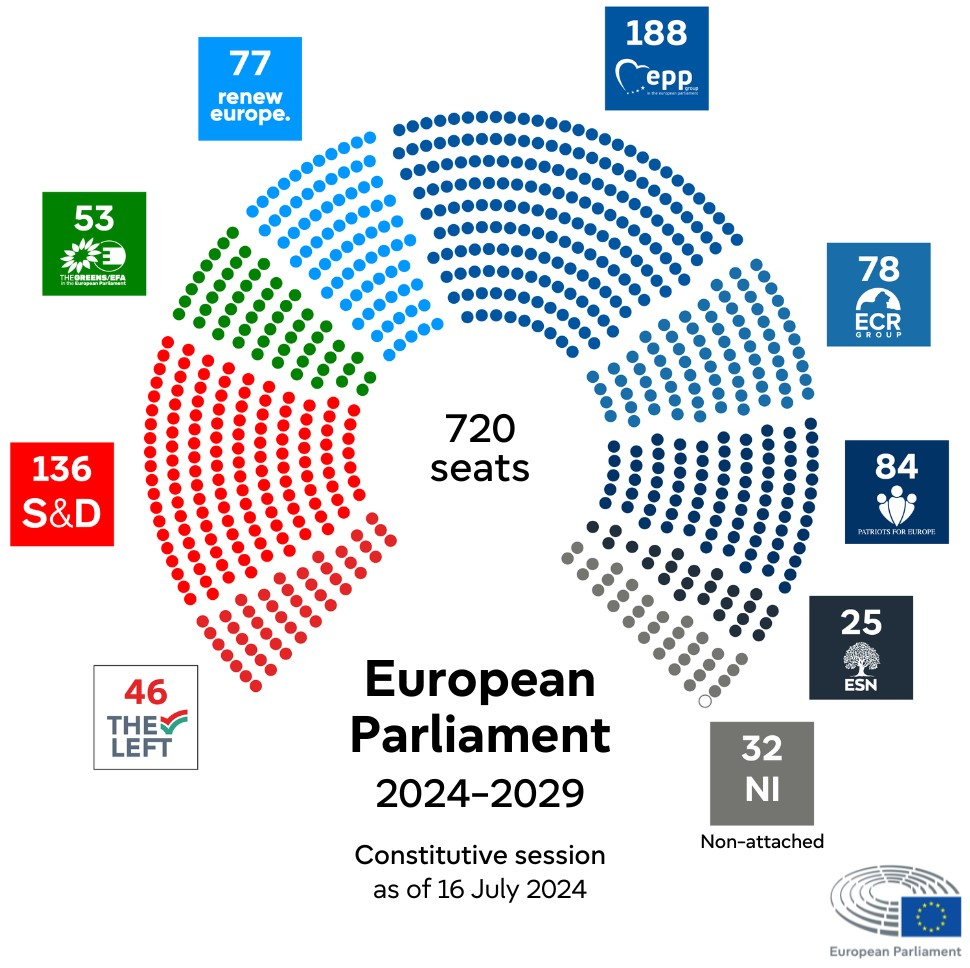
\includegraphics[width=4cm]{Bilder/EP_seats.jpg}
  \end{minipage}\hfill
  \begin{minipage}[c]{0.48\textwidth}
    \centering
    \ifthenelse{\equal{\fifthGroup}{Green}}{%
      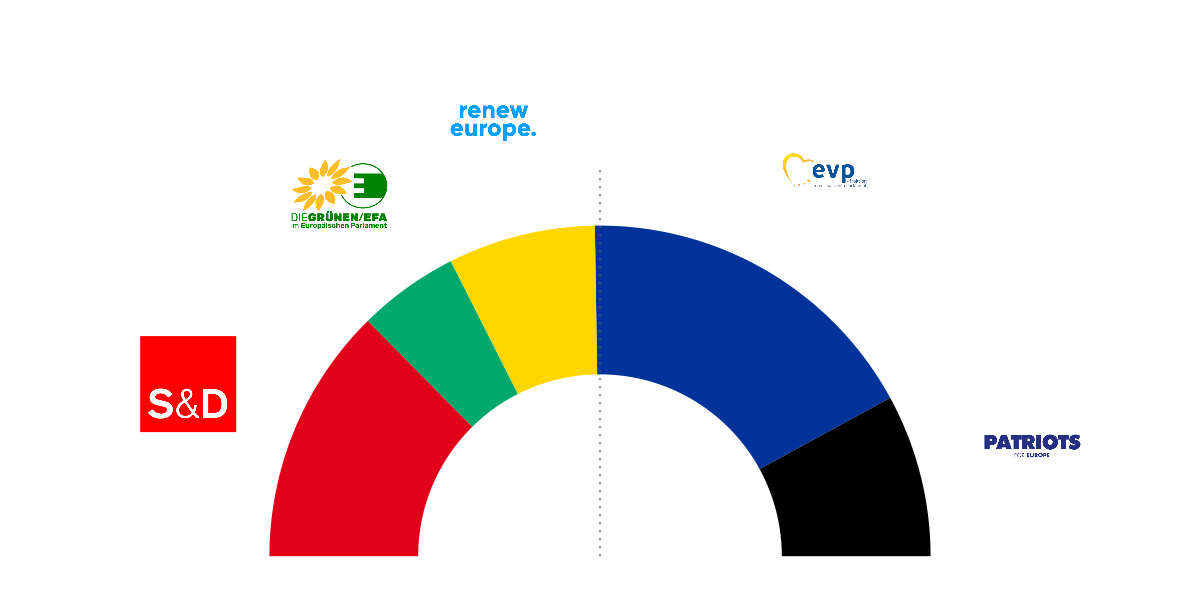
\includegraphics[width=6cm]{../../Scripts/semicircle_Green.png}%
    }{%
      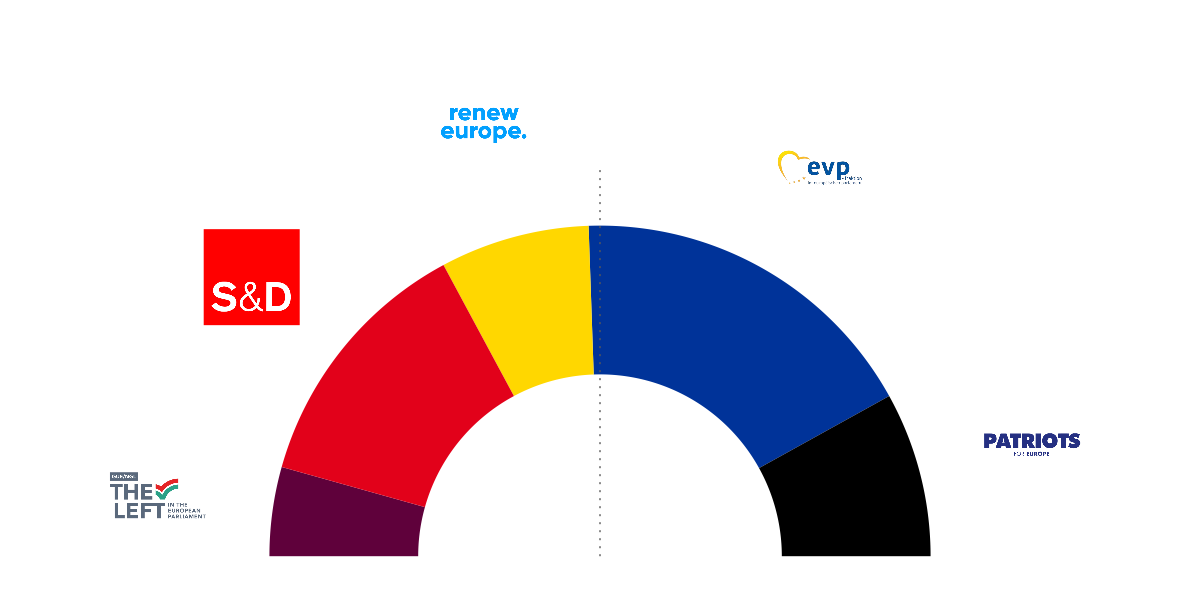
\includegraphics[width=6cm]{../../Scripts/semicircle_Left.png}%
    }%
  \end{minipage}
\end{figure}
\end{frame}


% ------------------ New: Individual statement slides ------------------
% Macro to select ideology statement by index
\newcommand{\ShowIdeology}[1]{%
	\IfEqCase{#1}{%
		{1}{\SharedIdeologyOne{\Fraktion}}%
		{2}{\SharedIdeologyTwo{\Fraktion}}%
		{3}{\SharedIdeologyThree{\Fraktion}}%
	}[]%
}

\newcommand{\ShowGoal}[1]{%
	\IfEqCase{#1}{%
		{1}{\SharedGoalOne{\Fraktion}{\Thema}}%
		{2}{\SharedGoalTwo{\Fraktion}{\Thema}}%
		{3}{\SharedGoalThree{\Fraktion}{\Thema}}%
	}[]%
}

% Helper macro for grid cells: fixed-width logo container + text
% Each cell uses fixed logo + text columns and a fixed row height for stable alignment
\newcommand{\GridCell}[2]{%
  \begin{minipage}[c]{0.49\textwidth}%
  \begin{minipage}[c]{0.05\textwidth}\centering
    \includegraphics[width=1cm]{Bilder/#1.png}%
  \end{minipage}\hspace{0.3\textwidth}%
  \begin{minipage}[c]{0.6\textwidth}\footnotesize\raggedright
    #2
  \end{minipage}%
  \end{minipage}%
}

% Helper macro for goal grid cells (with \Thema parameter)
\newcommand{\GridCellGoal}[2]{%
  \begin{minipage}[c]{0.49\textwidth}%
  \begin{minipage}[c]{0.05\textwidth}\centering
    \includegraphics[width=1cm]{Bilder/#1.png}%
  \end{minipage}\hspace{0.3\textwidth}%
  \begin{minipage}[c]{0.6\textwidth}\footnotesize\raggedright
    #2{\Thema}
  \end{minipage}%
  \end{minipage}%
}

% Helper macro to render a 2x2 grid of caucuses (excluding current)
% Usage: \ShowCaucusGrid{MACRO} where MACRO is the statement accessor (e.g., \SharedIdeologyOne)
\newcommand{\ShowCaucusGrid}[1]{%
  \ifthenelse{\equal{EVP}{\Fraktion}}{%
    % Current = EVP, show SD, RE, PfE, fifthGroup
    \GridCell{SD}{#1{SD}}\hfill
    \GridCell{RE}{#1{RE}}\par\vspace{0.4cm}
    \GridCell{PfE}{#1{PfE}}\hfill
    \ifthenelse{\equal{\fifthGroup}{Green}}{%
      \GridCell{Green}{#1{Green}}%
    }{%
      \GridCell{Left}{#1{Linke}}%
    }%
  }{%
    \ifthenelse{\equal{SD}{\Fraktion}}{%
      % Current = SD, show EVP, RE, PfE, fifthGroup
      \GridCell{EVP}{#1{EVP}}\hfill
      \GridCell{RE}{#1{RE}}\par\vspace{0.4cm}
      \GridCell{PfE}{#1{PfE}}\hfill
      \ifthenelse{\equal{\fifthGroup}{Green}}{%
        \GridCell{Green}{#1{Green}}%
      }{%
        \GridCell{Left}{#1{Linke}}%
      }%
    }{%
      \ifthenelse{\equal{RE}{\Fraktion}}{%
        % Current = RE, show EVP, SD, PfE, fifthGroup
        \GridCell{EVP}{#1{EVP}}\hfill
        \GridCell{SD}{#1{SD}}\par\vspace{0.4cm}
        \GridCell{PfE}{#1{PfE}}\hfill
        \ifthenelse{\equal{\fifthGroup}{Green}}{%
          \GridCell{Green}{#1{Green}}%
        }{%
          \GridCell{Left}{#1{Linke}}%
        }%
      }{%
        \ifthenelse{\equal{PfE}{\Fraktion}}{%
          % Current = PfE, show EVP, SD, RE, fifthGroup
          \GridCell{EVP}{#1{EVP}}\hfill
          \GridCell{SD}{#1{SD}}\par\vspace{0.4cm}
          \GridCell{RE}{#1{RE}}\hfill
          \ifthenelse{\equal{\fifthGroup}{Green}}{%
            \GridCell{Green}{#1{Green}}%
          }{%
            \GridCell{Left}{#1{Linke}}%
          }%
        }{%
          % Current = fifthGroup, show EVP, SD, RE, PfE
          \GridCell{EVP}{#1{EVP}}\hfill
          \GridCell{SD}{#1{SD}}\par\vspace{0.4cm}
          \GridCell{RE}{#1{RE}}\hfill
          \GridCell{PfE}{#1{PfE}}%
        }%
      }%
    }%
  }%
}

% Helper macro for goal grids (same pattern but macros need \Thema)
\newcommand{\ShowCaucusGridGoal}[1]{%
  \ifthenelse{\equal{EVP}{\Fraktion}}{%
    \GridCellGoal{SD}{#1{SD}}\hfill
    \GridCellGoal{RE}{#1{RE}}\par\vspace{0.4cm}
    \GridCellGoal{PfE}{#1{PfE}}\hfill
    \ifthenelse{\equal{\fifthGroup}{Green}}{%
      \GridCellGoal{Green}{#1{Green}}%
    }{%
      \GridCellGoal{Left}{#1{Linke}}%
    }%
  }{%
    \ifthenelse{\equal{SD}{\Fraktion}}{%
      \GridCellGoal{EVP}{#1{EVP}}\hfill
      \GridCellGoal{RE}{#1{RE}}\par\vspace{0.4cm}
      \GridCellGoal{PfE}{#1{PfE}}\hfill
      \ifthenelse{\equal{\fifthGroup}{Green}}{%
        \GridCellGoal{Green}{#1{Green}}%
      }{%
        \GridCellGoal{Left}{#1{Linke}}%
      }%
    }{%
      \ifthenelse{\equal{RE}{\Fraktion}}{%
        \GridCellGoal{EVP}{#1{EVP}}\hfill
        \GridCellGoal{SD}{#1{SD}}\par\vspace{0.4cm}
        \GridCellGoal{PfE}{#1{PfE}}\hfill
        \ifthenelse{\equal{\fifthGroup}{Green}}{%
          \GridCellGoal{Green}{#1{Green}}%
        }{%
          \GridCellGoal{Left}{#1{Linke}}%
        }%
      }{%
        \ifthenelse{\equal{PfE}{\Fraktion}}{%
          \GridCellGoal{EVP}{#1{EVP}}\hfill
          \GridCellGoal{SD}{#1{SD}}\par\vspace{0.4cm}
          \GridCellGoal{RE}{#1{RE}}\hfill
          \ifthenelse{\equal{\fifthGroup}{Green}}{%
            \GridCellGoal{Green}{#1{Green}}%
          }{%
            \GridCellGoal{Left}{#1{Linke}}%
          }%
        }{%
          \GridCellGoal{EVP}{#1{EVP}}\hfill
          \GridCellGoal{SD}{#1{SD}}\par\vspace{0.4cm}
          \GridCellGoal{RE}{#1{RE}}\hfill
          \GridCellGoal{PfE}{#1{PfE}}%
        }%
      }%
    }%
  }%
}
\begin{frame}{\Fraktionsname\ --- \IdeologyTitleOne}
\vspace{-0.15cm}
\begin{minipage}[c][0.85cm][c]{0.15\textwidth}\centering
  \includegraphics[height=0.8cm]{Bilder/\Fraktion.png}
\end{minipage}\hfill
\begin{minipage}[c][0.85cm][c]{0.82\textwidth}\small
  \ShowIdeology{1}
\end{minipage}
\vspace{0.08cm}
\hrule
\vspace{0.1cm}
{\footnotesize
  \ShowCaucusGrid{\SharedIdeologyOne}
}
\end{frame}

\begin{frame}{\Fraktionsname\ --- \IdeologyTitleTwo}
\vspace{-0.15cm}
\begin{minipage}[c][0.85cm][c]{0.15\textwidth}\centering
  \includegraphics[height=0.8cm]{Bilder/\Fraktion.png}
\end{minipage}\hfill
\begin{minipage}[c][0.85cm][c]{0.82\textwidth}\small
  \ShowIdeology{2}
\end{minipage}
\vspace{0.08cm}
\hrule
\vspace{0.1cm}
{\footnotesize
  \ShowCaucusGrid{\SharedIdeologyTwo}
}
\end{frame}

\begin{frame}{\Fraktionsname\ --- \IdeologyTitleThree}
\vspace{-0.15cm}
\begin{minipage}[c][0.85cm][c]{0.15\textwidth}\centering
  \includegraphics[height=0.8cm]{Bilder/\Fraktion.png}
\end{minipage}\hfill
\begin{minipage}[c][0.85cm][c]{0.82\textwidth}\small
  \ShowIdeology{3}
\end{minipage}
\vspace{0.08cm}
\hrule
\vspace{0.1cm}
{\footnotesize
  \ShowCaucusGrid{\SharedIdeologyThree}
}
\end{frame}

% Create three explicit slides for goals (1..3) — simplified, no loops
\begin{frame}[fragile]{\Fraktionsname\ --- \GoalTitleOne{\Thema}}
\vspace{-0.15cm}
\begin{minipage}[c][0.85cm][c]{0.15\textwidth}\centering
  \includegraphics[height=0.8cm]{Bilder/\Fraktion.png}
\end{minipage}\hfill
\begin{minipage}[c][0.85cm][c]{0.82\textwidth}\small
  \ShowGoal{1}
\end{minipage}
\vspace{0.08cm}
\hrule
\vspace{0.1cm}
{\footnotesize
  \ShowCaucusGridGoal{\SharedGoalOne}
}
\end{frame}

\begin{frame}[fragile]{\Fraktionsname\ --- \GoalTitleTwo{\Thema}}
\vspace{-0.15cm}
\begin{minipage}[c][0.85cm][c]{0.15\textwidth}\centering
  \includegraphics[height=0.8cm]{Bilder/\Fraktion.png}
\end{minipage}\hfill
\begin{minipage}[c][0.85cm][c]{0.82\textwidth}\small
  \ShowGoal{2}
\end{minipage}
\vspace{0.08cm}
\hrule
\vspace{0.1cm}
{\footnotesize
  \ShowCaucusGridGoal{\SharedGoalTwo}
}
\end{frame}

\begin{frame}[fragile]{\Fraktionsname\ --- \GoalTitleThree{\Thema}}
\vspace{-0.15cm}
\begin{minipage}[c][0.85cm][c]{0.15\textwidth}\centering
  \includegraphics[height=0.8cm]{Bilder/\Fraktion.png}
\end{minipage}\hfill
\begin{minipage}[c][0.85cm][c]{0.82\textwidth}\small
  \ShowGoal{3}
\end{minipage}
\vspace{0.08cm}
\hrule
\vspace{0.1cm}
{\footnotesize
  \ShowCaucusGridGoal{\SharedGoalThree}
}
\end{frame}

\begin{frame}{\glqq Zwischenprüfung\grqq}
\vspace{-1.5cm}
\begin{itemize}
	\item \href{\slidolink}{Slido zum \entwurf\ \& \Fraktionskuerzel}
\end{itemize}
\end{frame}

\begin{frame}{Rolleneinteilung}
\vspace{-1.5cm}
\begin{itemize}
	\item Ihr werdet nun einer der \anzahlcomm\ Ausschüsse zugeteilt
	\item Das Namensschild repräsentiert die Rolle, die ihr bis heute Nachmittag spielen werdet
\end{itemize}
\end{frame}

\begin{frame}{Ausschussgruppen}
\vspace{-1cm}
\begin{itemize}
    \item Trefft euch in den folgenden Ausschüssen:
	\begin{enumerate}
		\ausschussgruppen
	\end{enumerate}	    
    \item Besprecht den Gesetzesentwurf (insbesondere den Abschnitt eures Ausschusses) und an welchen Punkten es aus der Sicht der \Fraktionskuerzel -Fraktion noch Änderungsbedarf gibt.
\end{itemize}
\end{frame}


\begin{frame}{Ausschussgruppen}
\vspace{-1.5cm}
\begin{itemize}
    \item Legt euch auf einen (!) Änderungsantrag je Ausschussgruppe fest
    \item Bestimmt eine:n Ausschusssprecher:in, der:die eure Position und euren Änderungsantrag in der Ausschusssitzung kurz präsentiert
\end{itemize}
\end{frame}


\begin{frame}{So geht's weiter}
\vspace{-1.5cm}
\begin{itemize}
    \item \timeAuss: Ausschusssitzung \newline (Beratung der Änderungsanträge)
    \item \timeMittag: Mittagspause
    \item \timeFrakTwo: 2. Fraktionssitzung (Besprechung Ausschusssitzung \& finaler Änderungsantrag)
    \item \timeFinVerh: Finale Verhandlungsphase
    \item \timePlenar: Plenarsitzung \newline (Abschlussdebatte \& -abstimmung)
    \item \timeDebr: Debriefing \& Feedback
\end{itemize}
\end{frame}

\end{document}
